% Created 2025-04-05 Сб 01:12
% Intended LaTeX compiler: pdflatex
\documentclass[14pt,a4paper,oneside,openany]{book}
\usepackage[T2A]{fontenc}
% Настройка полей (левое: 30 мм, правое: 15 мм (можно 10 мм), верхнее: 20 мм, нижнее: 20 мм)
\usepackage[a4paper,top=20mm,bottom=20mm,left=30mm,right=15mm]{geometry}
% Межстрочный интервал 1.5 (14 пт рекомендуемый размер шрифта, можно задавать через документ или в настройках Overleaf)
\usepackage{setspace}
% \usepackage{mathptmx}
\onehalfspacing
\usepackage{cmap}

% русские буквы
\usepackage[utf8]{inputenc}
\usepackage[T2A]{fontenc}
\usepackage{svg}

\renewcommand{\contentsname}{Содержание}
\usepackage[main=russian,english]{babel}
\newcommand{\MyTOC}{%
  \chapter*{СОДЕРЖАНИЕ}%
  \setcounter{page}{6}
  \markboth{СОДЕРЖАНИЕ}{}%
  \vspace{-3.5cm}%
  {%
    \renewcommand{\contentsname}{}%
    \tableofcontents
  }%
}

% Абзацный отступ 1.25 см
\setlength{\parindent}{1.25cm}
\setlength{\parskip}{0pt}

% Нумерация страниц: арабскими цифрами, по центру нижней части
\usepackage{fancyhdr}
\pagestyle{plain}
\fancyhf{}
\cfoot{\thepage}

% Настройка заголовков через titlesec
\usepackage{titlesec}
% Заголовки глав: прописными буквами, полужирно, по центру, без точки в конце
\titleformat{\chapter}[hang]{\bfseries\Large\centering}{\thechapter}{1em}{}
% Заголовки разделов и подразделов – с абзацным отступом
\titleformat{\section}[hang]{\bfseries\large}{\thesection}{1em}{}
\titleformat{\subsection}[hang]{\bfseries}{\thesubsection}{1em}{}
\titlespacing{\chapter}{0pt}{0pt}{20pt}
\titlespacing{\section}{0pt}{12pt}{6pt}
\titlespacing{\subsection}{0pt}{6pt}{3pt}

% Настройка содержания: точечные лидеры между заголовками и номерами страниц
\usepackage{tocloft}
\renewcommand{\cftdotsep}{1}
\renewcommand{\cftchapleader}{\cftdotfill{\cftdotsep}}

% Подключаем отдельные конфигурационные файлы для списков, формул, таблиц и изображений
% \input{configs/config-lists.tex}
\usepackage{enumitem}
\setlist{nosep} % Убирает дополнительные отступы между элементами списков
\setlist[itemize]{leftmargin=*, label=\textbullet}
\setlist[enumerate]{leftmargin=*}
%%%%%%%%%%%%%%
% \input{configs/config-formulas.tex}
\usepackage{amsmath}
\numberwithin{equation}{chapter} % Формулы нумеруются по главам (например, (1.1), (1.2) и т.д.)
%%%%%%%%%%%%%
% \input{configs/config-tables.tex}
% Подключаем нужные пакеты для таблиц и оформления
\usepackage{booktabs}   % Для красивых горизонтальных линий (\toprule, \midrule, \bottomrule)
\usepackage{multirow}   % Для объединения ячеек по вертикали
\usepackage{float}
\usepackage{caption}    % Для \ContinuedFloat (продолжение таблицы)
\usepackage{longtable}
\usepackage{etoolbox}

\sloppy   % Избавляемся от переполнений
\clubpenalty=10000    % Запрещаем разрыв страницы после первой строки абзаца
\widowpenalty=10000   % Запрещаем разрыв страницы после последней строки абзаца

\usepackage{color}
\usepackage[svgnames]{xcolor}
\usepackage{listings}

\DeclareCaptionLabelSeparator{emdash}{\space---\space}  % пробел, длинное тире, пробел

\captionsetup[table]{position=t, singlelinecheck=false, justification=raggedright, labelsep=emdash, name=Таблица}
\captionsetup[figure]{position=b, singlelinecheck=false, labelsep=emdash, justification=centering, name=Рисунок}
% Настройка выравнивания заголовков

% Переключатель для смены выравнивания заголовков
\newcommand*\RightCaption{\captionsetup{justification=raggedleft}}
\newcommand*\LeftCaption{\captionsetup{justification=raggedright}}
%%%%%%%%%%%%

% Дополнительные пакеты
\usepackage[backend=biber,style=gost-numeric,sorting=none]{biblatex}
\usepackage{booktabs}

\newcommand\YAMLcolonstyle{\color{red}\mdseries}
\newcommand\YAMLkeystyle{\color{black}\bfseries}
\newcommand\YAMLvaluestyle{\color{blue}\mdseries}

\makeatletter

\newcommand\language@yaml{yaml}

\expandafter\expandafter\expandafter\lstdefinelanguage
\expandafter{\language@yaml}
{
  keywords={true,false,null,y,n},
  keywordstyle=\color{darkgray}\bfseries,
  basicstyle=\YAMLkeystyle\small,                                 % assuming a key comes first
  sensitive=false,
  comment=[l]{\#},
  morecomment=[s]{/*}{*/},
  commentstyle=\color{purple}\ttfamily,
  stringstyle=\YAMLvaluestyle\ttfamily,
  moredelim=[l][\color{orange}]{\&},
  moredelim=[l][\color{magenta}]{*},
  moredelim=**[il][\YAMLcolonstyle{:}\YAMLvaluestyle]{:},   % switch to value style at :
  morestring=[b]',
  morestring=[b]",
  literate =    {---}{{\ProcessThreeDashes}}3
                {>}{{\textcolor{red}\textgreater}}1
                {|}{{\textcolor{red}\textbar}}1
                {\ -\ }{{\mdseries\ -\ }}3,
}

% switch to key style at EOL
\lst@AddToHook{EveryLine}{\ifx\lst@language\language@yaml\YAMLkeystyle\fi}
\makeatother

\newcommand\ProcessThreeDashes{\llap{\color{cyan}\mdseries-{-}-}}
%%%%% Listing %%%%
%New colors defined below
\definecolor{codegreen}{rgb}{0,0.6,0}
\definecolor{codegray}{rgb}{0.5,0.5,0.5}
\definecolor{codepurple}{rgb}{0.58,0,0.82}
\definecolor{backcolour}{rgb}{0.95,0.95,0.92}
\definecolor{whitesmoke}{rgb}{0.96, 0.96, 0.96}

\lstdefinestyle{listingstyle}{
  backgroundcolor=\color{backcolour},
  commentstyle=\color{codegreen},
  keywordstyle=\color{magenta},
  numberstyle=\tiny\color{codegray},
  stringstyle=\color{codepurple},
  basicstyle=\ttfamily\footnotesize,
  breakatwhitespace=false,
  breaklines=true,
  captionpos=b,
  keepspaces=true,
  numbers=left,
  numbersep=5pt,
  showspaces=false,
  showstringspaces=false,
  showtabs=false,
  tabsize=4,
  inputencoding=utf8,
  extendedchars=true,
  literate=
    {а}{{\cyra}}1
    {б}{{\cyrb}}1
    {в}{{\cyrv}}1
    {г}{{\cyrg}}1
    {д}{{\cyrd}}1
    {е}{{\cyre}}1
    {ё}{\"{\cyre}}1
    {ж}{{\cyrzh}}1
    {з}{{\cyrz}}1
    {и}{{\cyri}}1
    {й}{{\cyrishrt}}1
    {к}{{\cyrk}}1
    {л}{{\cyrl}}1
    {м}{{\cyrm}}1
    {н}{{\cyrn}}1
    {о}{{\cyro}}1
    {п}{{\cyrp}}1
    {р}{{\cyrr}}1
    {с}{{\cyrs}}1
    {т}{{\cyrt}}1
    {у}{{\cyru}}1
    {ф}{{\cyrf}}1
    {х}{{\cyrh}}1
    {ц}{{\cyrc}}1
    {ч}{{\cyrch}}1
    {ш}{{\cyrsh}}1
    {щ}{{\cyrshch}}1
    {ъ}{{\cyrhrdsn}}1
    {ы}{{\cyrery}}1
    {ь}{{\cyrsftsn}}1
    {э}{{\cyrerev}}1
    {ю}{{\cyryu}}1
    {я}{{\cyrya}}1
    {А}{{\CYRA}}1
    {Б}{{\CYRB}}1
    {В}{{\CYRV}}1
    {Г}{{\CYRG}}1
    {Д}{{\CYR96}}1
    {Е}{{\CYRE}}1
    {Ё}{{\"{\CYRE}}}1
    {Ж}{{\CYRZH}}1
    {З}{{\CYRZ}}1
    {И}{{\CYRI}}1
    {Й}{{\CYRISHRT}}1
    {К}{{\CYRK}}1
    {Л}{{\CYRL}}1
    {М}{{\CYRM}}1
    {Н}{{\CYRN}}1
    {О}{{\CYRO}}1
    {П}{{\CYRP}}1
    {Р}{{\CYRR}}1
    {С}{{\CYRS}}1
    {Т}{{\CYRT}}1
    {У}{{\CYRU}}1
    {Ф}{{\CYRF}}1
    {Х}{{\CYRH}}1
    {Ц}{{\CYRC}}1
    {Ч}{{\CYRCH}}1
    {Ш}{{\CYRSH}}1
    {Щ}{{\CYRSHCH}}1
    {Ъ}{{\CYRHRDSN}}1
    {Ы}{{\CYRERY}}1
    {Ь}{{\CYRSFTSN}}1
    {Э}{{\CYREREV}}1
    {Ю}{{\CYRYU}}1
    {Я}{{\CYRYA}}1
}
\lstset{style=listingstyle} % для красивых листингов
%% Оформление подписей к листингам в стандарте вышки
\DeclareCaptionFormat{modifiedlst}{\lstlistingname~\thelstlisting~--~#3}
\captionsetup[lstlisting]{format=modifiedlst}

% Если язык не поддерживается (например, js) можно добавить свой https://tex.stackexchange.com/questions/89574/language-option-supported-in-listings
% или воспользоваться функцией без выделения синтаксиса через \lstset{style=listingstyle}
\lstdefinestyle{monochromestyle}{
  backgroundcolor=\color{whitesmoke},
  extendedchars=true,
  basicstyle=\footnotesize\ttfamily,
  showstringspaces=false,
  showspaces=false,
  numberstyle=\footnotesize,
  numbersep=9pt,
  breakatwhitespace=false,
  breaklines=true,
  captionpos=b,
  keepspaces=true,
  numbers=left,
  numbersep=5pt,
  showspaces=false,
  showstringspaces=false,
  showtabs=false,
  tabsize=4,
  inputencoding=utf8,
  extendedchars=true,
}

\usepackage[toc]{appendix}
\usepackage{tocloft}
\addto\captionsrussian{%
  \renewcommand{\appendixname}{ПРИЛОЖЕНИЕ}% This is good practice
}

\makeatletter

% Ваша команда \cyrtoc (оставляем как есть)
\def\cyrtoc#1{\ifcase #1\or А\or Б\or В\or Г\or Д\or Е\or Ж\or И\or К\or Л\or М\or Н\or П\or Р\or С\or Т\or У\or Ф\or Х\or Ц\or Ш\or Щ\or Э\or Ю\or Я\else \@ctrerr \fi}

\newcommand\originalappendix{}
\let\originalappendix\appendix

\renewcommand{\appendix}{%
  \label{pg:end} % For referencing the last page number if needed
  \originalappendix % Execute the original \appendix command (from appendix.sty with [toc] option)

  % 1. Redefine chapter numbering for appendices
  \renewcommand{\thechapter}{\cyrtoc{\value{chapter}}}
  % \appendixname is set to "ПРИЛОЖЕНИЕ" for Russian via \addto\captionsrussian in preamble

  % 2. Format chapter titles in the document body using 'titlesec'
}
\makeatother

\renewcommand{\contentsname}{Содержание}


\usepackage[utf8]{inputenc}
\usepackage[T2A]{fontenc}
\usepackage{graphicx}
\usepackage{longtable}
\usepackage{wrapfig}
\usepackage{rotating}
\usepackage[normalem]{ulem}
\usepackage{amsmath}
\usepackage{amssymb}
\usepackage{capt-of}
\usepackage{hyperref}
\author{Соломатин Роман Игоревич}
\date{}
\title{Разработка фреймфорка по автоматическому определению интентов}
\hypersetup{
 pdfauthor={Соломатин Роман Игоревич},
 pdftitle={Разработка фреймфорка по автоматическому определению интентов},
 pdfkeywords={},
 pdfsubject={},
 pdfcreator={Emacs 30.1 (Org mode 9.7.22)}, 
 pdflang={Russian}}
\usepackage{biblatex}
\addbibresource{~/Desktop/notes/org/bibliography.bib}
\begin{document}

\MyTOC

\chapter*{ТЕРМИНЫ И ОПРЕДЕЛЕНИЯ}
\label{sec:orge3707f8}
\textbf{AutoML} -- автоматическое машинное обучение.

\textbf{NLP} -- обработка естественного языка.

\textbf{NLU} -- понимание естественного языка.
\chapter*{Введение}
\label{sec:org52c6dc1}
\addcontentsline{toc}{chapter}{Введение}
В последние годы наблюдается бурный рост интереса к диалоговым системам на основе искусственного интеллекта (чат-ботам, голосовым помощникам и пр.). Так, по данным трендов, интерес к голосовым технологиям AI вырос почти втрое за пять лет\footnote{\url{https://www.verloop.io/blog/100-best-chatbot-statistics}}. Диалоговые системы внедряются в бизнес-процессы и повседневную жизнь, однако создание их интеллектуальной части – модели определения намерения пользователя (intent classification) – остается сложной задачей. Такой модуль является ключевым компонентом системы, позволяя автоматически выявлять цель запроса пользователя, но учет специфики различных доменов серьезно затрудняет разработку универсальной модели. Проектирование и тонкая настройка модели интентов требуют значительных экспертных усилий в области NLP и ML. Поэтому актуальной представляется автоматизация данного процесса – создание универсальных решений, способных уменьшить долю ручной работы и упростить разработку моделей классификации интентов. Автоматизированные подходы к машинному обучению (AutoML) обещают значительно сократить объем ручного труда за счет автоматического подбора оптимальных моделей и параметров, что особенно важно для быстро растущей области диалоговых систем.

На сегодняшний день для задачи классификации интентов накоплен внушительный арсенал методов. Традиционно применяются алгоритмы классического машинного обучения, такие как наивный tf-idf\autocite{joneskarensparck_statistical_1972}, а также подходы на основе k-ближайших соседей и ансамблевые методы (например, градиентный бустинг). С развитием глубокого обучения все более широко используются нейросетевые модели, таких как BERT\autocite{devlin_bert_2019}, которые достигают высоких показателей качества на задачах. Параллельно развиваются технологии AutoML, автоматизирующие выбор моделей и настройку гиперпараметров. Тем не менее, несмотря на прогресс отдельных компонентов, целостных универсальных AutoML-фреймворков, специально ориентированных на определение интентов пользователя, предложено немного. Существующие решения зачастую требуют участия эксперта для каждой новой предметной области, что указывает на необходимость разработать более обобщенный подход.

В связи с этим актуальной является проблема отсутствия универсального, масштабируемого и эффективного AutoML-решения для классификации интентов, способного автоматически адаптироваться к разным доменам без глубокого участия человека-эксперта.

\textbf{Цель исследования} заключается в разработке такого универсального AutoML-фреймворка, который способен автоматически подбирать оптимальные модели и их конфигурации для классификации интентов пользователя. Разработанное решение будет протестировано на различных корпусах данных (наборы пользовательских запросов), а его эффективность сопоставлена с результатами ручной настройки моделей, чтобы оценить выигрыш от автоматизации.

Для достижения поставленной цели в работе решены следующие задачи:
\begin{enumerate}
\item разработка архитектуры и программной реализации AutoML-фреймворка для классификации интентов;
\item экспериментальное испытание фреймворка на нескольких корпусах данных, относящихся к различным предметным областям;
\item сравнение результатов, полученных с помощью AutoML-фреймворка, с качеством моделей, настроенных вручную, и анализ эффективности предлагаемого подхода.
\end{enumerate}

\textbf{Практическая значимость} работы состоит в том, что созданный AutoML-фреймворк может быть непосредственно применен при разработке реальных диалоговых систем – чат-ботов, голосовых ассистентов, систем клиентской поддержки – и других NLP-приложений. Использование такого инструмента позволит ускорить внедрение новых сервисов и снизить порог вхождения для разработчиков за счет автоматизации подбора оптимальной модели под конкретный набор интентов.

\textbf{Научная новизна} исследования определяется интеграцией современных методов автоматизированного машинного обучения в единой специализированной архитектуре, ориентированной на задачу классификации интентов. В предлагаемом решении объединяются передовые подходы, включая трансформерные модели и методы обучения с малым количеством примеров, в рамках одного AutoML-фреймворка. Такое сочетание технологий нацелено на достижение высокой точности и устойчивости модели при минимальном ручном вмешательстве, что ранее не было реализовано в полной мере для задачи определения интентов пользователя.
\chapter{ОБЗОР ПРЕДМЕТНОЙ ОБЛАСТИ}
\label{sec:org5cd0b2a}
\section{Определение намерений пользователя}
\label{sec:org02b3e55}
Классификация намерений –  это задача сопоставления высказывания пользователя с предопределенной меткой намерения (семантической категорией цели пользователя). Например, запрос “Какая погода будет завтра?” может быть классифицирован как запрос погоды. Эта способность является ключевым компонентом понимания естественного языка (NLU) в диалоговых системах, позволяя чат-ботам, виртуальным помощникам и другим агентам искусственного интеллекта понимать, чего хочет пользователь, и соответствующим образом реагировать. Классификация намерений уходит корнями в ранние разговорные диалоговые системы (например, телефонное обслуживание клиентов) и с тех пор получила повсеместное распространение в самых разных областях - от личных помощников и ботов поддержки клиентов до систем медицинских и юридических консультаций.

Ранние методы были основаны на правилах, которые разрабатывались вручную, или на классическом машинном обучении с добавлением дополнительных функций. Однако с развитием области преобладать стали статистические методы, которые основываются на анализе данных. Сначала они использовали традиционные алгоритмы машинного обучения, а затем — методы глубокого обучения. Также мы наблюдаем расширение сферы применения: от простой классификации с закрытым набором параметров, когда каждый запрос должен относиться к одному из известных намерений, до более сложных сценариев. Например, к многоцелевой классификации, обнаружению намерений с открытым доменом или открытым набором параметров (когда запрос не соответствует ни одному из известных намерений), а также к распознаванию намерений с минимальным количеством попыток или вообще без них с помощью мощных генеративных моделей.
\subsection{KNN}
\label{sec:orgb3a1a91}
\begin{enumerate}
\item MLKNN
\label{sec:orgcc851fd}
Тут будет описание метода \autocite{zhang_mlknn_2007}
\item DNNC
\label{sec:org55d4e21}
Тут будет описание метода \autocite{zhang_discriminative_2020}
\item Hierarchical small navigable small worlds
\label{sec:org543ff21}
Тут будет описание метода \autocite{malkov_efficient_2018}
\end{enumerate}
\subsection{Классификация}
\label{sec:org4694102}
\begin{enumerate}
\item Бустинг
\label{sec:org3b7c0fa}
Тут будет описание метода catboost \autocite{dorogush_catboost_2018,prokhorenkova_catboost_2018}
\item Трансформеры
\label{sec:orgdb31345}
Тут будет описание метода \autocite{reimers_sentencebert_2019,devlin_bert_2019,vaswani_attention_2017}. Peft\autocite{han_parameterefficient_2024}, LoRa\autocite{hu_lora_2021}
\end{enumerate}
\section{Методы автоматического машинного обучения}
\label{sec:org3e28c3d}
Автоматизированное машинное обучение (AutoML) относится к автоматизации полного процесса применения методов машинного обучения для решения реальных задач. Вместо того чтобы вручную выбирать алгоритмы, настраивать гиперпараметры, разрабатывать архитектуры моделей и создавать признаки, система AutoML автоматически принимает эти решения на основе данных. Мотивация для развития AutoML вытекает из бурного роста применения машинного обучения и стремления {}<<демократизировать>>{} машинное обучение – сделать современные техники доступными даже для неспециалистов. Модели машинного обучения зачастую чувствительны к множеству параметров (тип модели, архитектура, настройки гиперпараметров, предварительная обработка признаков и так далее), и нахождение оптимальной конфигурации часто требует кропотливого перебора даже для экспертов. Эта проблема особенно заметна в глубоком обучении, где выбор правильной архитектуры сети и стратегии обучения может определять конечное качество модели. Цель AutoML – автоматизировать принятие этих решений, позволяя пользователю просто предоставить данные, а система подбирает оптимальную модель. Данный обзор литературы предоставляет академический анализ AutoML с основным упором на его применение в обработке естественного языка (NLP), а также включает как фундаментальные работы, так и последние разработки. Мы рассмотрим историческую эволюцию и мотивации AutoML, ключевые технические компоненты, ведущие фреймворки и системы, особенности применения AutoML в задачах NLP (например, классификация текстов, маркировка последовательностей, языковое моделирование), сравнительный анализ производительности и существующие бенчмарки, а также новые тенденции и направления исследований (например, интеграция с фундаментальными моделями, обучение с малым количеством примеров, объяснимость моделей). Обзор ссылается на рецензируемые публикации и академические источники.

\begin{itemize}
\item LAMA\autocite{vakhrushev_lightautoml_2022}
\item AutoGluon\autocite{erickson_autogluontabular_2020}
\item H2O\autocite{ledell_h2o_2020}
\item TPOT
\item TextBrew\autocite{desai_textbrew_2022}
\end{itemize}
\section{Текстовые аугментации}
\label{sec:org4640e02}
\begin{itemize}
\item Intent-augmentation \autocite{hu_exploring_2024}
\item Few-shot detection \autocite{hou_fewshot_2021}
\item Dspy \autocite{khattab_dspy_2023}
\end{itemize}
\chapter{ПРОЕКТИРОВАНИЕ}
\label{sec:org91635ce}

\begin{figure}[h]
\centering
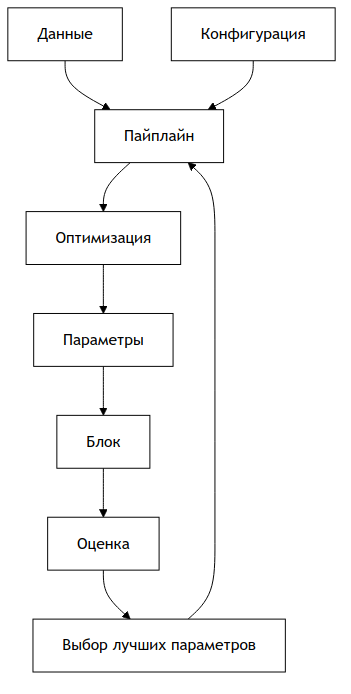
\includegraphics[width=0.6\textwidth,height=0.5\textheight]{img/mermaid/framework_schema.png}
\caption{\label{fig:framework_schema}Схема фреймворка}
\end{figure}
\chapter*{Заключение}
\label{sec:org1459497}
\printbibliography[title=СПИСОК\spaceИСПОЛЬЗОВАНЫХ\spaceИСТОЧНИКОВ]
\end{document}
